\documentclass{beamer}
%\usepackage{colortbl}
\usepackage[latin1]{inputenc}
\usepackage{comment}
%\usetheme{Warsaw}
\usetheme{Frankfurt}
\usecolortheme{dove}
\usepackage[absolute,overlay]{textpos} 
\usepackage{booktabs}
\usepackage{color}
\usepackage{threeparttable}
\usepackage{multirow}
%\usepackage[table]{xcolor}
%\definecolor{tableShade}{HTML}{F1F5FA}


\title[Epistasis in GWAS]{Genetic interactions in eQTL studies}
\date{}
\begin{document}

\AtBeginSection[]
{
  \begin{frame}<beamer>
    \frametitle{Outline}
    \tableofcontents[currentsection,currentsubsection]
  \end{frame}
}

\begin{frame}
\titlepage
\end{frame}


\section{Epistasis}
\subsection{}

\begin{frame}{Epistasis}
\begin{definition}
{\color{orange} The effect on the phenotype caused by locus A depends on the genotype at locus B }
%{\tiny \color{white} \newline - Carlborg and Haley 2004 }
\end{definition}
\end{frame}

\begin{frame}{Examples}

\begin{figure}[htb]
 \centering
 \begin{minipage}[c]{0.38\textwidth}
  \centering
{\tiny
\begin{tabular}{cccc}
& AA & Aa & aa \\\hline
BB & $2\alpha + 2\beta$ & $\alpha + 2\beta$ & $2\beta$ \\
Bb & $2\alpha + \beta$ & $\alpha + \beta$ & $\beta$ \\
bb & $2\alpha$ & $\alpha$ & $0$ \\
&&&\\
\multicolumn{4}{l}{Additive + additive (not epistatic)}\\

\end{tabular} }
 \end{minipage}
 \begin{minipage}[c]{0.38\textwidth}
 \includegraphics[width=\textwidth]{additive.jpg}
 \end{minipage}
 \end{figure}

\begin{figure}[htb]
 \centering
 \begin{minipage}[c]{0.38\textwidth}
   \centering
{\tiny
\begin{tabular}{cccc}
& AA & Aa & aa \\\hline
BB & $\alpha$ & $\alpha$ & $\alpha$ \\
Bb & $\alpha$ & $\alpha$ & $\alpha$ \\
bb & $\alpha$ & $\alpha$ & $\beta$ \\
&&&\\
\multicolumn{4}{l}{Canalisation (epistatic)}\\
\end{tabular} }
 \end{minipage}
 \begin{minipage}[c]{0.38\textwidth}
 \includegraphics[width=\textwidth]{canalisation.jpg}
 \end{minipage}
\end{figure}
\end{frame}

\begin{frame}{Two dimensional GWAS}
\begin{center}
\includegraphics[width=7cm]{2dscan.png} \\
{\tiny Carlborg 2004}
\end{center}
\end{frame}

\begin{frame}{Impact of LD on observed variance}
\begin{center}
\includegraphics[width=5cm]{gpmaps_ld.png} \\
\end{center}
\end{frame}

\section{Computational solutions}
\subsection{}

\begin{frame}{The problem}
Number of interactions: \\
\begin{equation}
n(n-1) / 2 \nonumber
\end{equation}
500000 SNPs $\rightarrow$ 125 billion interactions \\
\begin{itemize}
\item PLINK performs 5000 tests per second $\rightarrow$ 3 years
\item FastEpistasis performs 36000 tests per second $\rightarrow$ 5 months
\item Optimised C code 125000 tests per second $\rightarrow$ 6 weeks
\item Parallelised on 8-core CPU $\rightarrow$ 5 days
\end{itemize}
\end{frame}


\begin{frame}{CPUs and hitting the `power wall'}
\begin{itemize}
\item All electrical power consumed eventually radiates as heat
\item Processor speed requires more power to improve
\begin{itemize}
\item Increased heat
\item Increased circuit resistance
\item Instability
\end{itemize}
\end{itemize}
\end{frame}

\begin{frame}{CPU limits}
\begin{center}
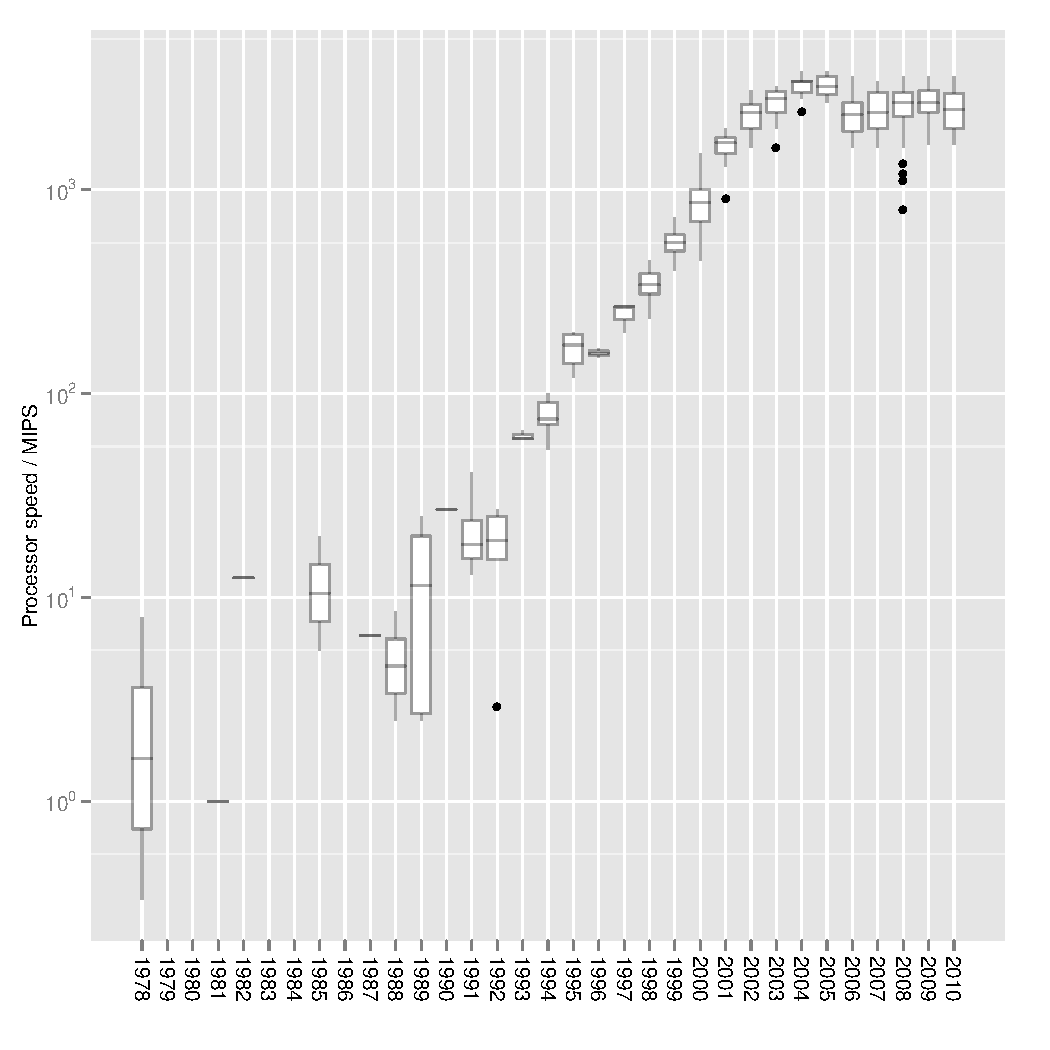
\includegraphics[height=7cm]{clockspeed.pdf}
\end{center}
\end{frame}

\begin{frame}{CPU limits}
\begin{center}
\includegraphics[height=6cm]{clockrates.png}
\end{center}
\end{frame}

\begin{frame}{Graphics cards}
	\includegraphics[height=2.5cm]{cpugpu.png}
	\begin{itemize}
		\item Many cores that can process data simultaneously
		\item But all the cores are extremely simple
		\begin{itemize}
			\item Tiny L1 cache
			\item Little communication between cores
			\item Each core is relatively slow
			\item Cores are divided into local groups, all of which must do the same thing
		\end{itemize}
	\end{itemize}
\end{frame}


\begin{frame}{GPU speeds}
	\begin{center}
		\includegraphics[height=7cm]{gpuoptimisation.pdf}
	\end{center}
\end{frame}

\begin{frame}{epiGPU}
	\begin{itemize}
		\item http://sourceforge.net/projects/epigpu/
		\item Free
		\item Open source
		\item Windows, Mac, Linux
		\item NVIDIA and ATI graphics cards
	\end{itemize}
\end{frame}


% mention epiGPU

\section{Thresholds}
\subsection{}

\begin{frame}{The curse of dimensionality}
As the dimensionality of the search increases the background noise drowns out all real biological signals
\end{frame}

\begin{frame}{Linkage disequilibrium}
\begin{center}
\includegraphics[width=10cm]{ld.png}
\end{center}
\begin{itemize}
\item SNPs are correlated $\rightarrow$ tests are not independent
\item Bonferroni correction is overly stringent
\end{itemize}
\end{frame}

\begin{frame}{A general formula for 2D thresholds?}
\begin{center}
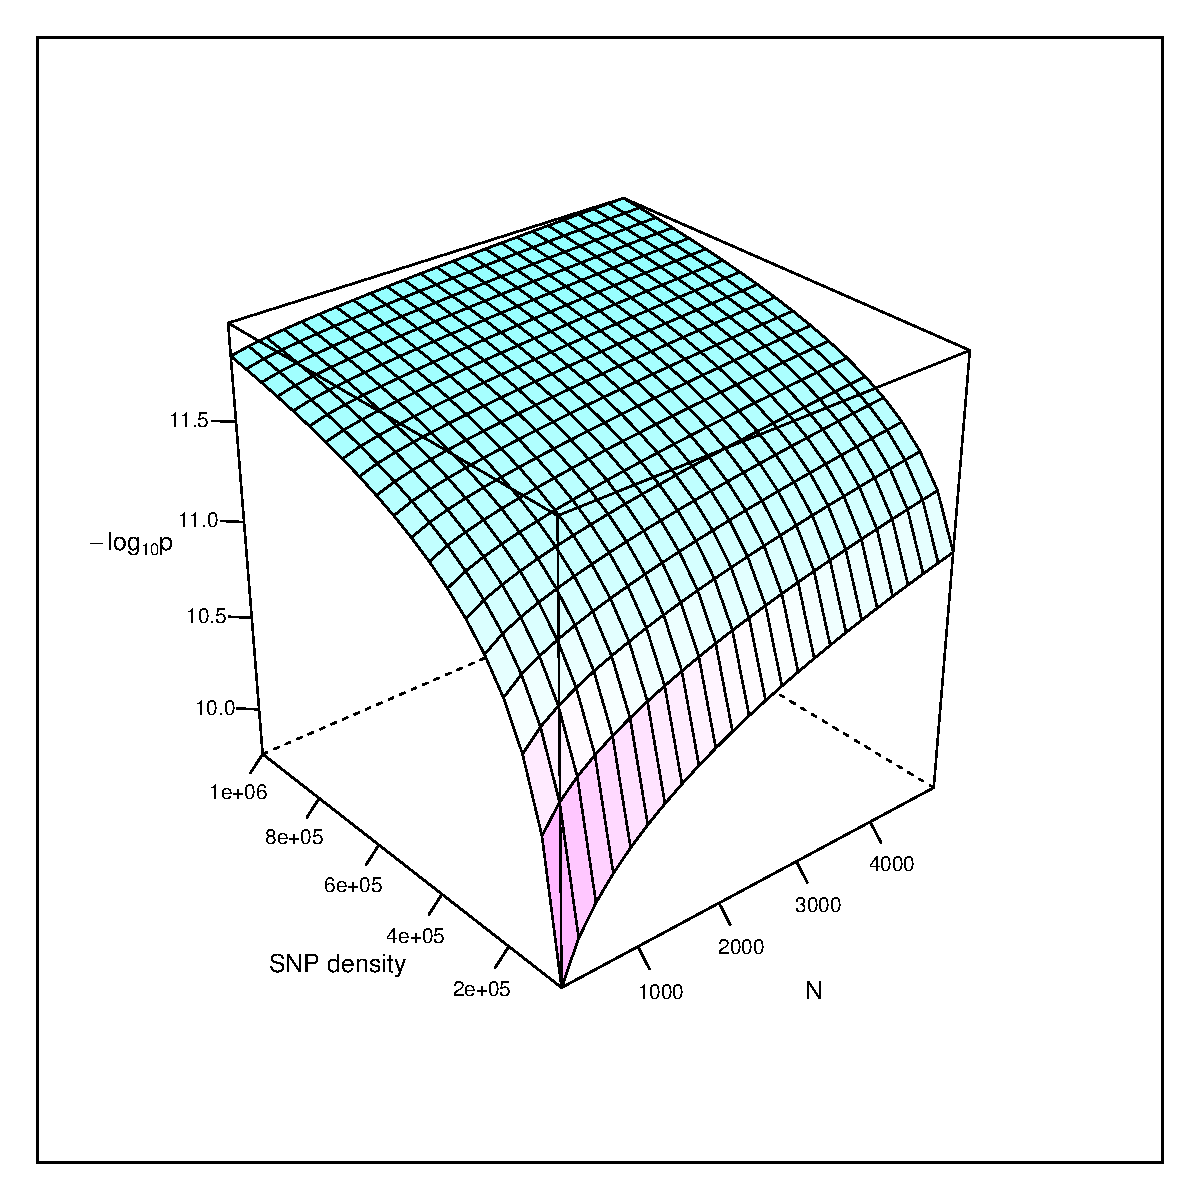
\includegraphics[height=7cm]{threshold_function.pdf}
\end{center}
\end{frame}


\section{2D eQTL}
\subsection{}

\begin{frame}{Are epistatic effects controlling gene expression?}
	\begin{itemize}
		\item Lower level traits: less polygenic?
		\item Typically eQTLs have very large effects
		\item Better power for epistatic searches, despite multiple testing burden
		\item Make inferences about genetic architecture
		\item Make inferences about disease aetiology 
	\end{itemize}
\end{frame}

\begin{frame}{Details}
	\begin{itemize}
		\item Study design:
		\begin{itemize}
			\item 846 healthy Australian adults
			\item 546,192 SNPs
			\item 5380 gene expression probes from whole blood
		\end{itemize}
		\item Plan:
		\begin{itemize}
			\item Correct phenotypes for fixed and polygenic effects
			\item Do exhaustive search for 2 locus epistasis for residuals on each probe
			\item Parallelise search across 100x GPU cluster
		\end{itemize}
	\end{itemize}
\end{frame}

\begin{frame}{Thresholds}
	\begin{itemize}
		\item 1641 complete scans were performed on permuted phenotype
		\item Threshold predicted to be: \textbf{11.648}
		\item Empirical estimate: \textbf{11.632}
		\item Average correlation between 5380 probes: \textbf{0.265}
		\item Overall threshold: $-\log_{10}p =$ \textbf{16.5}
	\end{itemize}
\end{frame}

\begin{frame}{Very preliminary results}
	\begin{itemize}
	\item Is there much non-additive variance?
	\item 71 probes have significant eQTLs after filtering for:
	\begin{itemize}
	\item Threshold of 16.5
	\item Additive variance $\leq$ 60\% of total genetic variance
	\item Relatively common SNPs (must have samples for all 9 genotype classes)
	\item No LD between interacting SNPs
	\end{itemize}
	\item Total of 140 significant independent loci
	\end{itemize}
\end{frame}

\begin{frame}{Very preliminary results}
\begin{itemize}
\item Proportion of the phenotypic variance explained:
\begin{itemize}
\item Total genetic: range 8.4\% - 17.1\%
\item Total non-additive: range 3.5\% - 9.2\%
\end{itemize}
\item 14\% cis-cis
\item 69\% cis-trans
\item 17\% trans-trans
\end{itemize}
\end{frame}

\begin{frame}{Some examples}
\begin{center}
\includegraphics[height=7.5cm]{epistasis_examples}
\end{center}
\end{frame}

\end{document}


